%
% latex-sample.tex
%
% This LaTeX source file provides a template for a typical research paper.
%

%
% Use the standard article template.
%
\documentclass{article}

% The geometry package allows for easy page formatting.
\usepackage{geometry}
\geometry{letterpaper}

% Load up special logo commands.
\usepackage{doc}

% Package for formatting URLs.
\usepackage{url}

% Packages and definitions for graphics files.
\usepackage{graphicx}
\usepackage{epstopdf}
\DeclareGraphicsRule{.tif}{png}{.png}{`convert #1 `dirname #1`/`basename #1 .tif`.png}

\usepackage{float}

%
% Set the title, author, and date.
%
\title{An Analysis of Distributed Test Suites With Load Balancing and Sharing}
\author{Michael Camara, Colton McCurdy, Gary Miller, \& Herbie Torrance}
\date{}

%
% The document proper.
%
\begin{document}

% Add the title section.
\maketitle

% Add an abstract.
\abstract{
This research focuses on the utilizing distributed testing to make the execution of large test suites more efficient. The key trade-offs for taking a distributed approach to testing are be identified and the impacts on using a distributed approach are analyzed. This paper will mainly focus on comparing two distributed test systems, Test Load Balancer (TLB), and our own system, Distributed Test Sharer (DTS).

% Add various lists on new pages.
\pagebreak
\tableofcontents

% Start the paper on a new page.
\pagebreak

%
% Body text.
%
\section{Introduction}
\label{introduction}

Testing is often considered to be one of the most important components of the software development cycle and therefore it is important to conduct a thorough and correct test suite on a software system. Many large software systems are subject to testing that can take several hours and potentially longer to execute, which can be very costly. For example, in situations where a system's test suite can take several hours or even days to execute, and one of the tests that is not executed early in the testing process fails, the cost of identifying this failure can be exceptionally high. For this reason, approaches to decreasing the cost of executing test suites is a very popular topic in software development. One of approaches to successfully reducing the cost associated with testing a system is to use distributed testing. This is an approach in which test cases are distributed or scattered across many different nodes in a network, executed locally on that given node, and the result of the test case is then returned across the network. The focus of this research is to identify, analyze, and report the results of experiments conducted on distributed testing using two different systems, Test Load Balancer (TLB) and Distributed Test Sharer (DTS). It is hypothesized that by distributing test cases and executing them in parallel on several independent nodes, the overall cost of executing a full test suite can be reduced due to the increase of computational resources and evaded the limitations experienced with computing on a single node.

\section{Background On Distributed Testing}

In order to conduct an analysis on using a distributed approach to testing, more research on the trade-offs associated with the topic was conducted. First, it is important to understand situations in which distributed testing may be beneficial; the most obvious being when a test suite takes several hours or days to execute. It also may be necessary to conduct distributed testing if the the system of focus must be tested on different web browsers or sites, in the case of a web-based application, or even on different operating systems. In either case, it may be difficult or costly to executing these tests on a single node and therefore distributed the tests to other nodes may be beneficial. 

Next, it is essential to identify both the benefits and drawbacks of testing in a distributed fashion. Some of the key benefits associated with distributed testing is that less computation is required on the CPU in which the system is executed on, which allows more work to be done locally and is potentially a large benefit in a situation where it is necessary to execute other processes alongside the test suite. More importantly, the goal is to reduce the runtime of the test suite by executing several test cases in parallel and is an exceptionally more feasible task when using multiple CPUs. One of the most common ways in which the increase in performance is a achieved is by diminishing the cost of dependencies. Tests cases that are dependent on another case often have larger costs because their result or even execution may not occur until another case is completed. By using distributed testing, these dependent test cases can be isolated to a particular node that is responsible for executing the group of dependent cases while other nodes can execute other independent cases that otherwise would have been waiting in a queue if centralized testing was used. This situation is a clear example in which a distributed approach would be more beneficial that a centralized approach.

Though it is clear the distributed testing may be beneficial to use there certainly are drawbacks and challenges that exist with this approach. The greatest of these drawbacks is the cost of communication required to transfer data over a network from one node to another. In order to execute a test case at a remote location, either the code to execute the test must exist at the remote location or the code must be sent across the network. This is a potentially costly situation if the required code is large and takes up a lot of memory. The situation where the code already exists at the remote location is often unlikely and therefore the test code usually must be transferred to the node that will execute it, therefore it must be determined whether communication costs of distributed testing out weighs the computational and time costs associated with executing the tests locally. Another drawback associated with distributed testing is that it is dependent on a network, which in some cases may be unavailable. If a system uses a distributed test suite and it is unable to gain access to a network, then there is no way to run the tests until a network becomes available. Another unfavorable situation may occur if there are fewer remote nodes available than required. In a situation such as this, both the communications costs and computational limitations may be experienced because all of the data is transferred to a number of locations that cannot execute the tests in a time that justifies distributing the tests.

Alongside the drawbacks of distributing testing, several challenges exist with this approach as well. One of the key challenges associated with distributed testing is the concept of load sharing versus load balancing. Load sharing occurs when the tests or load are sent to several nodes to be executed without any restrictions on how the load is allocated. Load balancing is a more complex approach in which the allocation of the load is sent to nodes such that each node is doing an equivalent amount of work. This allows the load to be executed more efficiently because it prevents situations in which a particular node is doing a significantly greater amount of work than others or a particular node is doing little to no work at all. It is quite evident that load balancer is a more favorable approach to take, but the complexity associated with it is much larger. For example, consider a situation in which a test case is dependent on another, in this case a load balancing system must not only consider the amount of load to allocate to each node, but also when certain components of the load need to be allocated. 

\section{Overview of Related Work}
\subsection{Existing Systems}

Though distributed testing is a popular and rapidly developing topic in the software industry, not many systems that use his approach exist and work correctly. This is due to the fact that it is not only a relatively new concept, but the complexity of building a system that can run tests on a system and efficiently distribute them to remote nodes is exceptionally high. One existing system that successfully does this is named Test Load Balancer (TLB). TLB claims to support testing of every language on every platform and partitions the tests into subsets that can be executed in parallel on different physical or virtual machines. These subsets are executed in such a way that they all start at the same time and finish at almost the same time as well, therefore the overall time is takes to execute all of the tests can be divided by the number of test subsets that are generated. TLB assures that a particular node will execute only a number of tests proportional to the total number of test divided by the number of available nodes and guarantees mutual exclusion and collective exhaustion of test execution, meaning that no test will be executed more than once and every test will be executed. The TLB system is comprised on two main components, the first of which is a server that is responsible for storing test data and the second is the balancer that partitions and orders the execution of tests. By storing test data, the TLB system will reorder the execution of tests with each run based on previous results. This is a extremely beneficial feature because tests that are known to fail will be executed earlier to avoid unnecessary downtime time resulting from failing tests being executed later. Though it is very important to note that this is only achievable by using tests that are independent of one another which is not always the cases. Unfortunately, large systems very often have test cases that are dependent on other tests and systems such as these are usually examples that would benefit from using distributed testing opposed to centralized testing. Also, this method can not guarantee the order in which tests are executed due to its fail early approach to executing test, therefore tests must not only be independent of other tests but also independent of the order in which they are executed.

\subsection{Distributed Test Sharer}
In order to understand and further evaluate the trade-offs associated with distributed testing, we developed a novel system named the Distributed Test Sharer (DTS).  This system was created using the Java programming language and consists of two main classes: \texttt{Delegator} and \texttt{CustomServer}.  The relationship between these classes is illustrated in Figure \ref{dtsdiagram}, with communication facilitated by Java Remote Method Invocation (RMI) and use of an FTP server.  The following section will outline the steps performed by DTS to distribute JUnit tests located on the \texttt{Delegator} node to any number of \texttt{CustomServer} nodes, which run the tests and return the results obtained.

\begin{figure}[H]
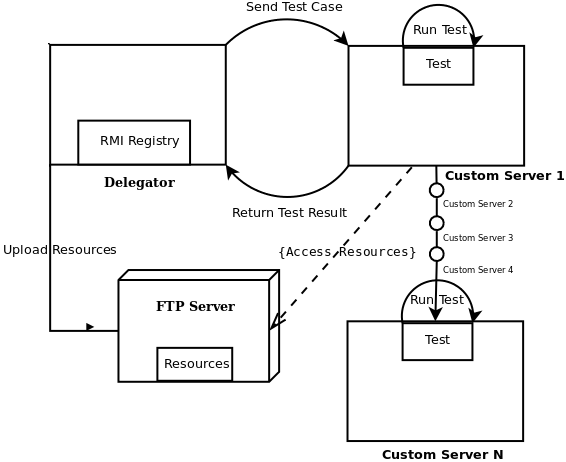
\includegraphics[width = \textwidth]{DTS_Diagram.png}
\caption{Architecture of the Distributed Test Sharer (DTS).}
\label{dtsdiagram}
\end{figure}

Before starting the system, the user is expected to furnish all of the JUnit test cases and any associated resources needed to run those test cases.  All files will be placed in the \texttt{ftpserver} directory, or one of its subdirectories.  The top level of this directory can be filled with any non-class files or directories that might be required for test suite execution.  For instance, the SchemaAnalyst test suite uses a \texttt{config} directory that contains various text files filled with different properties.  In this example, the user would place the entire \texttt{config} directory immediately inside the \texttt{ftpserver} directory.  Further nested in the \texttt{ftpserver} directory is a \texttt{resources} directory, which contains  \texttt{bin}, \texttt{lib}, \texttt{test\_singles} and \texttt{test\_suites} subdirectories.  For simplicity, the user should put the entirety of the directory containing their compiled classes in the \texttt{bin} directory.  Continuing with the SchemaAnalyst example, this would involve placing the \texttt{org}, \texttt{paper}, and \texttt{parsedcasestudy} directories into the \texttt{ftpserver/resources/bin} directory, which are usually located in that system's \texttt{build} directory.  All \texttt{jar} files used by the desired tests should be placed in the \texttt{lib} directory.  Finally, any individual JUnit test cases can be put in the \texttt{ftpserver/resources/test\_singles} directory, while any test suites (those that reference multiple JUnit test cases, like an \texttt{AllTests} class) can be put in the \texttt{ftpserver/resources/test\_suites} directory.


DTS execution begins on the side of the \texttt{Delegator} with a few preliminary steps.  First, several system properties are programmatically altered. These include \texttt{java.security.policy}, which is set to a custom policy that grants all permissions to any nodes that attempt to connect to the \texttt{Delegator} through Java RMI.  Although a more stringent policy would generally be recommended to improve the security of the system, this was deemed appropriate for the purpose of prototyping the system with fewer obstacles.  Further, the \texttt{java.rmi.server.hostname} property is set to the internet protocol (IP) address of the \texttt{Delegator}, which is retrieved through the command line interface at program execution.  This specifies the given IP address for use with any registry that is subsequently created, allowing remote nodes to find it.

Next, a Java RMI registry is created using a port number that is currently hard coded as 12345.  This port number was chosen because it resides in the range of acceptable ports for the machines used for experimentation, and generally is not assigned to any other system processes.  A new instance of \texttt{Delegator} is then created and linked to the registry through use of the \texttt{rebind()} method, binding the object with a key of "Delegator."  This will allow \texttt{CustomServer} nodes to access some of the methods offered by \texttt{Delegator} in future steps.

Both the \texttt{Delegator} and \texttt{CustomServer} classes extend \texttt{UnicastRemoteObject}, which allows them to be bound to and retrieved from a Java RMI registry.  It facilitates the dynamic creation of stubs for such objects, obviating the static method used in previous versions of Java.  Each class also implements an interface that extends \texttt{Remote}: \texttt{DelegatorInterface} and \texttt{CustomServerInterface}.  The \texttt{Remote} marker interface is further required to successfully bind to the registry, and it allows for type checking of remote object invocations at compile time.

After the registry is created, an FTP server is created using the Apache FtpServer framework.  This framework was chosen because it allows programmatic creation of an FTP server using Java, instead of relying on a third-party application that would need to be run and configured separately.  Various settings are adjusted during this step, such as establishing a user name and password, setting the port and host address, and enabling concurrent logins.  Most importantly, the home directory for the FTP server is set to the \texttt{ftpRootDir} variable, which is currently hard coded to the local \texttt{ftpserver} directory where the test cases and resources were previously placed.  Any users that connect successfully with the server will then have immediate access to this directory and any nested directories contained within it.

The final preliminary step taken by \texttt{Delegator} is the creation of a list of JUnit test cases.  Both the \texttt{ftpserver/resources/test\_singles} and \texttt{ftpserver/resources/test\_suites} are traversed recursively to locate all nested \texttt{class} files, which are saved as \texttt{File} objects and stored into separate global \texttt{LinkedLists}: \texttt{testSingleList} and \texttt{testSuiteList}.

After these steps are completed by the \texttt{Delegator}, it waits until the user enters the carriage return character to continue.  During this wait, remote nodes can connect to the \texttt{Delegator} by running the \texttt{CustomServer} class.  Importantly, two command line arguments must be specified at execution: the IP address of the \texttt{Delegator}, followed by the server's own IP address.  Ideally, multicasting would be used by the \texttt{Delegator} to broadcast its address, allowing the \texttt{CustomServers} to locate it automatically.  While this might be pursued in the future, the current implementation requires the \texttt{Delegator's} IP address to be known.  

Once started, the \texttt{CustomServer} sets the system RMI policy in the same manner as done by the \texttt{Delegator}.  Additionally, it will set the \texttt{java.system.class.loader} system property to a \texttt{CustomClassLoader}.  This class extends a \texttt{URLClassLoader} and allows access to some of the normally protected methods through use of reflection.  For now, it simply sets the classpath to the local \texttt{bin} and \texttt{lib} directories.  Next, the \texttt{CustomServer} will locate the registry on the \texttt{Delegator}, using the IP address previously specified, and obtain a remote reference to the bound \texttt{Delegator} object using the \texttt{Naming.lookup()} method.  Using this reference, it will call the \texttt{rebindServer()} method to bind the \texttt{CustomServer} to the registry.  This is repeated for each \texttt{CustomServer} node until they are all bound to the registry.

After all \texttt{CustomServers} are created and connected, then the user will enter the carriage return character on the \texttt{Delegator} node to continue execution.  The \texttt{Delegator} will first call the remote \texttt{updateClassLoader()} method for each of the \texttt{CustomServers}.  This will add all of the relevant \texttt{class} directories and \texttt{jar} files to the classpath of each \texttt{CustomServer}, accessible via FTP protocol and the FTP server previously created.  Additionally, all of the non-class files previously placed in the \texttt{ftpserver} directory on the \texttt{Delegator} node are actively retrieved through communication with the FTP server and stored locally on each server node.  Although efforts were made to obviate the need to store any files on the server, this was deemed a critical step to ensure that subsequent tests could be run successfully.

Next, the \texttt{Delegator} creates \texttt{TestAgent} objects for each \texttt{CustomServer}.  These agents extend the \texttt{Thread} class and implement \texttt{Runnable}, allowing multiple agents to run their respective methods concurrently on separate threads.  The \texttt{run()} method will simply do a remote call to the \texttt{runTest()} method for its assigned \texttt{CustomServer}, sending a test case and storing the \texttt{Result} generated by the server into the same \texttt{ConcurrentLinkedQueue}.  These agents are further placed into another \texttt{ConcurrentLinkedQueue} for subsequent access by the \texttt{Delegator}.

Once these agents are created, the \texttt{Delegator} will sequentially iterate first through the \texttt{testSingleList}, and then through the \texttt{testSuiteList}.  With the single test cases, each \texttt{File} in the list is assigned as-is to an agent in the queue, provided that agent is not currently active.  The \texttt{run()} method of the agent is then started, sending the test to the assigned \texttt{CustomServer}.  If the agent is active, then it is placed back into the queue and the next agent is checked, continuing in that manner.  This load sharing approach ensures that each \texttt{TestAgent}, and therefore each \texttt{CustomServer}, is always running a single test case at all times.  This process is similarly repeated while iterating through the test suites, with some additional steps.  The test suite \texttt{File} is first converted into a byte array, which is then converted into a \texttt{Class} object using a \texttt{SimpleClassLoader}.  This class loader simply overrides the \texttt{defineClass()} method of a generic \texttt{ClassLoader}, allowing this conversion to take place.  Next, the test suite is further converted into an array of \texttt{Class} objects by retrieving all test cases listed under the \texttt{SuiteClasses} annotation in the suite.  This array, containing all of the individual test cases in the suite, is iterated through in the same manner described previously, performing load sharing using the previously created agents.

On the \texttt{CustomServer}, there are two \texttt{runTest()} methods: one has a \texttt{File} parameter, while one has a \texttt{Class} parameter.  The method for \texttt{Class} objects simply executes the static \texttt{JUnitCore.runClasses()} method on that object, which returns a \texttt{Result} object.  This \texttt{Result} object contains all of the details about the successes and failures from running the test, and is returned to the caller.  The \texttt{runTest()} method for \texttt{File} objects first converts the \texttt{File} to bytes, and then to a \texttt{Class} object, finally using the same \texttt{JUnitCore.runClasses()} method to run the test.  This is performed by the \texttt{CustomServer} to lessen the computation required on the \texttt{Delegator} as much as possible.  In both cases, running the tests is only possible due to the previously implemented \texttt{CustomClassLoader}.  This allows the JVM to automatically retrieve any needed \texttt{class} or \texttt{jar} files via communication with the FTP server on the \texttt{Delegator} without any prompting from the user, and without needing to copy those files to the \texttt{CustomServer} node.

The \texttt{Delegator} continues to perform load sharing, assigning test cases to \texttt{TestAgents}.  The agents continue to store the \texttt{Result} objects returned from the \texttt{runTest()} method of each \texttt{CustomServer} into the same \texttt{ConcurrentLinkedQueue}.  Once all tests have been assigned, and all \texttt{Results} have been retrieved, then the each \texttt{Result} is parsed and the total number of successes and failures are displayed for the user.  Each failure is further elaborated to show why a test case might have failed.  This completes the process used by the Distributed Test Sharer, with all tests located on the \texttt{Delegator} having been executed by separate, remote nodes.

\section{Experimentation Protocol}

This section will explain the experimentation process that was followed for collecting data on the two systems.


\section{Analysis of Results}

This section will report and analyze the data that was collected from the experiment.

\section{Challenges}

Various challenges were encountered while developing the Distributed Test Sharer, with many of these challenges revolving around the use of Java RMI for communication between nodes.  There were a variety of different settings and properties that I didn't originally know about, despite using this technique in a previous assignment.  These included either setting the RMI host name and security policy through the \texttt{-Djava} command line parameter, or using the \texttt{System.setProperty()} method programmatically.  Omitting these steps produced a variety of different, confusing errors, and required much troubleshooting to figure out how to fix them.  There were also problems getting the RMI to work on the computers in Alden Hall, which ultimately prevented those computers from being used in our experiments.  Originally, these problems arose from the fact that the Java RMI registry would occasionally use a random port number instead of the one specified in the source code.  This created much confusion originally, since the Java API includes various method signatures that require a port number parameter; yet it seemed as though such specification did not have the expected effect.  Ultimately, using a custom \texttt{SocketServerFactory} and adjusting the parameters for the \texttt{UnicastRemoteObject} constructor fixed those initial problems involving randomly assigned ports.  However, new problems arose with remote objects being removed from the registry after binding, perhaps due to some garbage collection issue.  These problems were not present during testing of DTS on personally owned computers, and unfortunately they could not be resolved despite significant time investment.

Another challenge with DTS was getting the tests to run on a separate node without error, and specifically without needing to copy over any files to the servers.  I used a custom \texttt{URLClassLoader} to originally overcome this challenge, which is a vital component to the system.  Although this allows the JVM to access the FTP server for \texttt{class} and \texttt{jar} file, it doesn't redirect the paths used for other kinds of files.  For instance, the SchemaAnalyst test suite makes use of a \texttt{config} directory that contains various properties files.  Although I could specify the exact FTP URL for the class loader to locate this directory, the test cases would not find it when they ran on the server.  I tried to adjust the system property for the current working directory (\texttt{user.dir}), among other fixes, but could never bypass this error completely.  Ultimately, in order to get the tests to work as expected, I need to add a step to the \texttt{updateClassLoader()} method on the \texttt{CustomServers} to retrieve and store some files from the FTP server.  This was unfortunate, since a notable benefit of this system is the lack of resource overhead for the servers; but it was necessary in order to have a functional system within our time constraints.  This general issue with file dependencies further complicated running DTS on complex systems like \texttt{ant-ivy} and \texttt{tomcat}, despite the accommodations made to DTS.  The prevented DTS to be run on similar systems as TLB, and it would be one of the first areas of improvement if development on this system were to continue.

\section{Conclusion}

This section concludes the findings and topics outlined throughput the report.

% Generate the bibliography.
\bibliography{latex-sample}
\bibliographystyle{unsrt}

\end{document}
